\chapter{Matrix II: Nonlinear Equations}\label{ch:matrix-nonliear}

\normalsize

In the previous chapter, we numerically solved a linear equation $A \vb{x} = \vb{b}$.  This equation can be also written as a problem of finding zeros (root-finding) of a linear function
\begin{equation}\label{eq:linear_zero}
\vb{f}(\vb{x}) \equiv A \vb{x} - \vb{b} = 0
\end{equation}
where $\vb{f}$, $\vb{x}$, and $\vb{b}$ are column vectors, and $A$ a matrix.  We are able to solve this kind of problems by Gaussian eliminations or its extension.  However, those methods are limited to linear equations and cannot solve non-linear equations.
For example,  a function of vector $\vb{x}=(x_1,x_2,x_3)$
\begin{eqnarray}
\vb{f}(\vb{x}) = \begin{bmatrix} -2 x_1 + 2 x_2 - 1\\ 3 x_1 - x_2 - x_1 x_3 + 3\\ x_1 x_2 - x_3  + 2\end{bmatrix}
\end{eqnarray}
is nonlinear (the product of multiple elements such as $x_1 x_2$ makes it nonlinear) and cannot be written in the linear form $A \vb{x} = \vb{b}$.
 
Although many physics problems are linear, non-linear problems are becoming increasingly important in many areas of science.  In this chapter,
we develop numerical methods to solve nonlinear equations $\vb{f}(\vb{x})=0$, which is a multivariable version of root finding problem.  We have discussed the root finding methods for nonlinear equations of single variable in Chapter \ref{ch:root-finding}.  The bisection method obviously won't work for multivariable systems.  However, the Newton-Raphson and secant method can be extended to multivariable nonlinear systems.

\subsection{Multi-Dimensional Newton-Raphson Methods}

\begin{figure}
\centering
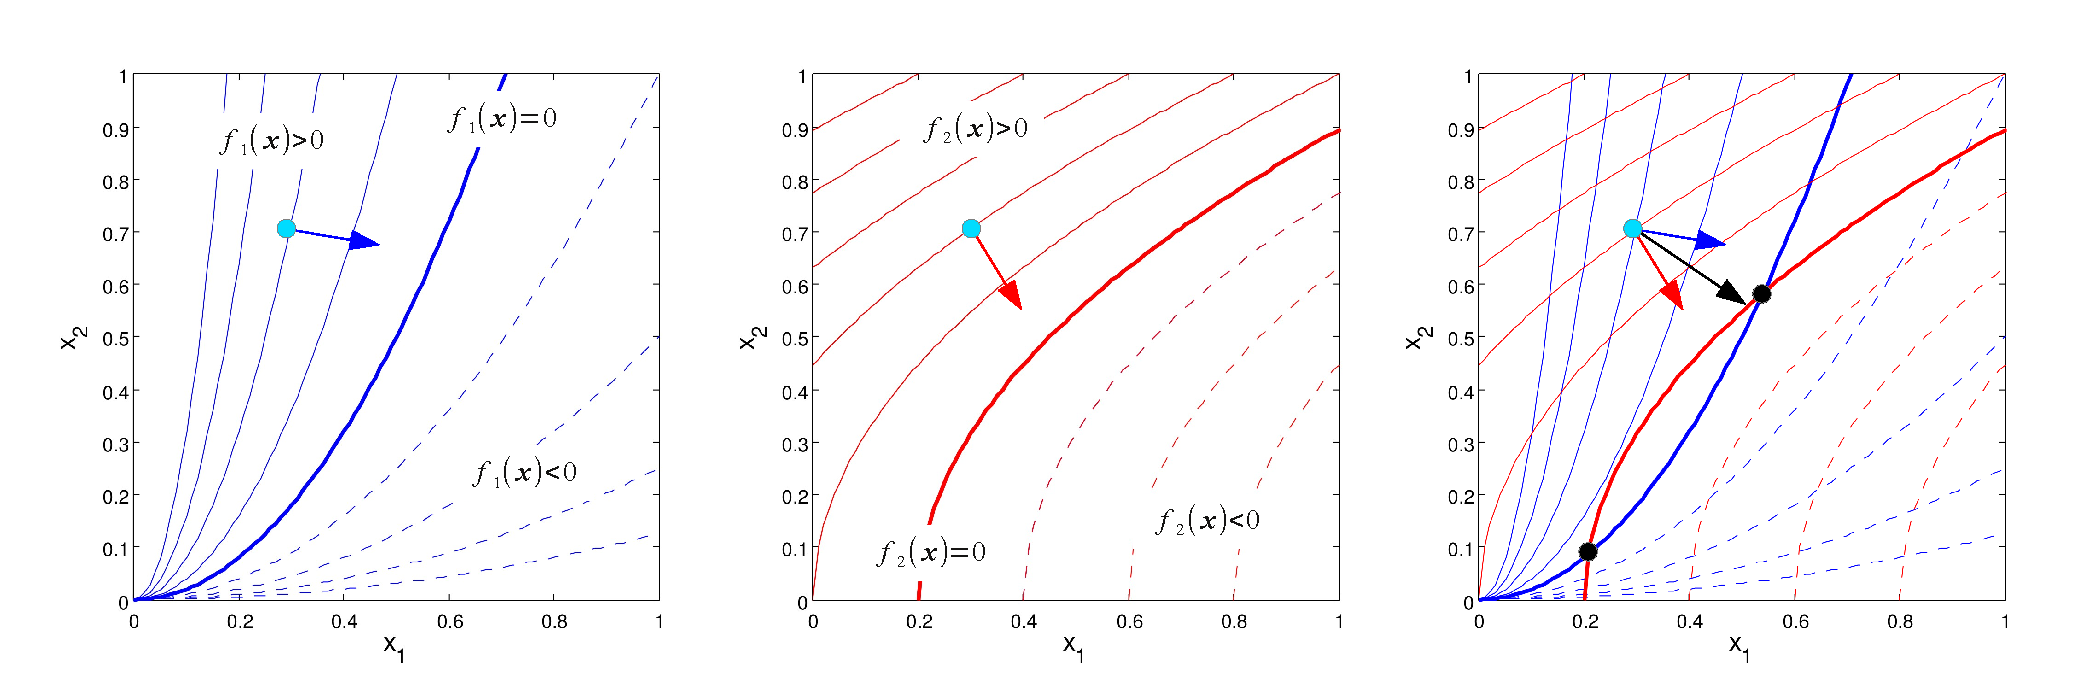
\includegraphics[width=6in]{09.matrix2/2d-newton.pdf}
\caption{Diagram of 2D Newton-Raphson step. \textit{Left}: The landscape of $f_1(\vb{x})$.  The thick line indicates the nullcline $f_1(\vb{x})=0$.
Starting at the initial guess (circle), $-\grad f_1(\vb{x})$ (arrow) tells the steepest descent toward the nullcline. \textit{Center}:  The landscape for $f_2(\vb{x})$.  Similar to the left panel, the arrow point to the nullcline $f_2(\vb{x})=0$. \textit{Right}:
The superimpose of the left and center panel.  The crossing points of two nullclines are the solutions.  The vector sum of two steepest descent direction (black arrow) approximately points the solution.}\label{fig:2d_newton}
\end{figure}

To begin with, we consider two variables case.  The equations we want to solve is written explicitly with the components as
\begin{subequations} \label{eq:2d_roots}
\begin{eqnarray}
f_1 (\vb{x}) &=& 0 \label{eq:2d_roots_a}\\
f_2 (\vb{x}) &=& 0 \label{eq:2d_roots_b}
\end{eqnarray}
where 
\begin{equation}
\vb{x} = \begin{bmatrix} x_1 \\ x_2 \end{bmatrix}
\end{equation}
\end{subequations}
Figures \ref{fig:2d_newton} illustrate the landscape of $f_i (\vb{x})$ in contours.  The thick lines are nullclines (\ref{eq:2d_roots_a}) and \eqref{eq:2d_roots_b}. The solutions of Eq. \eqref{eq:2d_roots} are crossing points of the two nullclines. See the right panel of the illustration. 

Starting with an initial guess $x^{(0)}$ (a blue circle), we want to move toward the solution. The steepest descent directions determined by $-\grad f_i$ point to the corresponding nullclines. (See the left and middle panel.)  These directions not necessarily point to a root.  However, the sum of the two steepest descent directions, $\grad f_1 + \grad f_2$ approximately points to the root as the right panel of Fig. \ref{fig:2d_newton} shows. Using these slopes,
\begin{subequations}
\begin{eqnarray}
f_1 (\vb{x}) - f_1(\vb{x}^{(0)}) &\approx& -\grad f_1(\vb{x}^{(0)}) \cdot (\vb{x} - \vb{x}^{(0)}) \\
f_2 (\vb{x}) - f_2(\vb{x}^{(0)}) &\approx& -\grad f_2(\vb{x}^{(0)}) \cdot (\vb{x} - \vb{x}^{(0)})
\end{eqnarray}
\end{subequations}
Since $f_1(\vb{x})=f_2(\vb{x})=0$, we can estimate the root by solving
\begin{subequations}
\begin{eqnarray}
\grad f_1(\vb{x}^{(0)}) \cdot (\vb{x} - \vb{x}^{(0)}) &=& -f_1(\vb{x}^{(0)}) \\
\grad f_2(\vb{x}^{(0)}) \cdot (\vb{x} - \vb{x}^{(0)}) &=& -f_2(\vb{x}^{(0)})
\end{eqnarray}
\end{subequations}
for $\vb{x}$.  This is a linear equation and can be solved by the methods discussed in the previous chapter. We write this equation in a matrix form :
\begin{equation}
\begin{bmatrix}
\displaystyle\frac{\partial f_1}{\partial x_1} & \displaystyle\frac{\partial f_1}{\partial x_2} \\[12pt]
\displaystyle\frac{\partial f_2}{\partial x_1} & \displaystyle\frac{\partial f_2}{\partial x_2} \end{bmatrix}
\begin{bmatrix} x_1 - x_1^{(0)} \\ x_2 - x_2^{(0)} \end{bmatrix}
=
\begin{bmatrix}f_1(\vb{x}^{(0)}) \\f_2(\vb{x}^{(0)}) \end{bmatrix}
\end{equation}
The 2-by-2 matrix is just a Jacobian matrix evaluated at $\vb{x}^{(0)}$. Inverting the Jacobian matrix, the approximate solution is
$\vb{x} = \vb{x}^{(0)} - J^{-1} \vb{f}(\vb{x}^{(0)})$.  Although formally we use the inverse matrix, remember that we don't need to calculate $J^{-1}$ to find the numerical solution as we learned in the previous Chapter.  Once we find the new position $\vb{x}$, use it as the new starting point and repeat the procedure until $||\vb{x}^{(n)}-\vb{x}^{(n-1)}|| < \text{tolerance}$.

Now, we generalize the above result to the $N$-dimension
\begin{equation}
\vb{f}(\vb{x}) = \begin{bmatrix} f_1(\vb{x}) \\ f_2(\vb{x}) \\ \vdots \\ f_N({\vb{x}}) \end{bmatrix}
, \qquad \text{where} \quad
\vb{x} = \begin{bmatrix} x_1 \\ x_2 \\ \vdots \\ x_N \end{bmatrix}
\end{equation}
We want to find zeros of this function.   Starting with an initial guess $\vb{x}^{(0)}$, we predict the root using the ``slope''.   Expanding the function in a Taylor series about $\vb{x}^{(0)}$,
\begin{equation}
\vb{f}(\vb{x}) = \vb{f}(\vb{x}^{(0)}) + J^{(0)} (\vb{x}-\vb{x}^{(0)}) + \cdots
\end{equation}
where $J$ is the Jacobian matrix defined by
\begin{equation}
J^{(0)}_{ij} = \left . \frac{\partial f_i(\vb{x})}{\partial x_j} \right |_{\vb{x}=\vb{x}^{(0)}}
\end{equation}
Ignoring the higher order terms, the root finding equation is now
\begin{equation}
\vb{f}(\vb{x}) = \vb{f}(\vb{x}^{(0)}) + J^{(0)}\, (\vb{x}-\vb{x}^{(0)}) = 0
\end{equation}
and its solution is
\begin{equation}
\vb{x}^{(1)} = \vb{x}^{(0)} - \left (J^{(0)}\right )^{-1} \vb{f}(\vb{x}^{(0)})
\end{equation}
This is the root suggested by the Newton-Raphson's method.  If $|\vb{f}(\vb{x}^{(1)})| < \text{tolerance}$, we have found a solution.
If not, we continue the iterative procedure:
\begin{equation}
\vb{x}^{(n+1)} = \vb{x}^{(n)} - \left( J^{(n)}\right )^{-1} \vb{f}(\vb{x}^{(n)})
\end{equation}

If the initial guess is far from the solution, the Newton-Raphson method often fails. This instability can be avoided by reducing the jump size.  For example, we modify the above iteration process slightly by multiplying $0< \alpha < 1$ to each step.
\begin{equation}
\vb{x}^{(n+1)} = \vb{x}^{(n)} - \alpha \left( J^{(n)}\right )^{-1} \vb{f}(\vb{x}^{(n)}).
\end{equation}
With  a small step length, you might expect more iterations.  That is not the case for many cases.  

\begin{myalgobox}
   \Algorithm{Multivariate Newton-Raphson Method}\label{algo:gaussian_elimination}
   \begin{enumerate}
      \item Choose a step factor $\alpha \in (0, 1]$.
      \item Set an initial guess $\vb{x}^{(0)}$.
      \item Repeat the following procedure starting with $n=0$.
      \item Solve $A \vb{y} = \vb{b}$ using Gaussian elimination or LU decomposition methods, where $A = J^{(n)}$ and $\vb{b}=-\vb{f}(\vb{x}^{(n)})$.
      \item The new solution is given by $\vb{x}^{(n+1)}= \vb{x}^{(n)}+\alpha \vb{y}$.
      \item If $| \vb{f}(\vb{x}^{(n+1)}) | < \text{tolerance}$.  Then, $\vb{x}^{(n+1)}$ is the solution.
      \item If not, increment $n$ and repeat from step 5.
   \end{enumerate}
\end{myalgobox}

\bigskip
\begin{example}\label{ex:newton_raphson_2d}

We solve a two-dimensional nonlinear equation
\begin{subequations}
\begin{eqnarray}
2 x + 3 x y &=& 1\\
x y + 3 y &=& -1
\end{eqnarray}\label{eq:nonlinear_2d}
\end{subequations}
using the Newton-Raphson method. See  Program \ref{prog:newton_raphson_2d}.  When $\alpha=1$ is used, the output ends up with \texttt{NaN}.  When $\alpha=0.1$ is used , 698 iterations are needed to get a desired accuracy ($10^{-8}$).  With a larger step size $\alpha=0.5$, more iterations are needed to get the same answer.   Figure \ref{fig:newton_raphson_2d} shows how the iteration approaches to the solution.   The final values of the iteration agree with the exact solution $x=\displaystyle\frac{-1+\sqrt{7}}{2}$ and $y=\displaystyle\frac{-5+\sqrt{7}}{9}$.
 

\begin{mybox}

\small
\begin{verbatim}
Iternations = 698
Solution= 8.228757e-01, -2.615832e-01
   Exact= 8.228757e-01, -2.615832e-01
\end{verbatim}
\normalsize
\end{mybox}

\begin{figure}
\centering
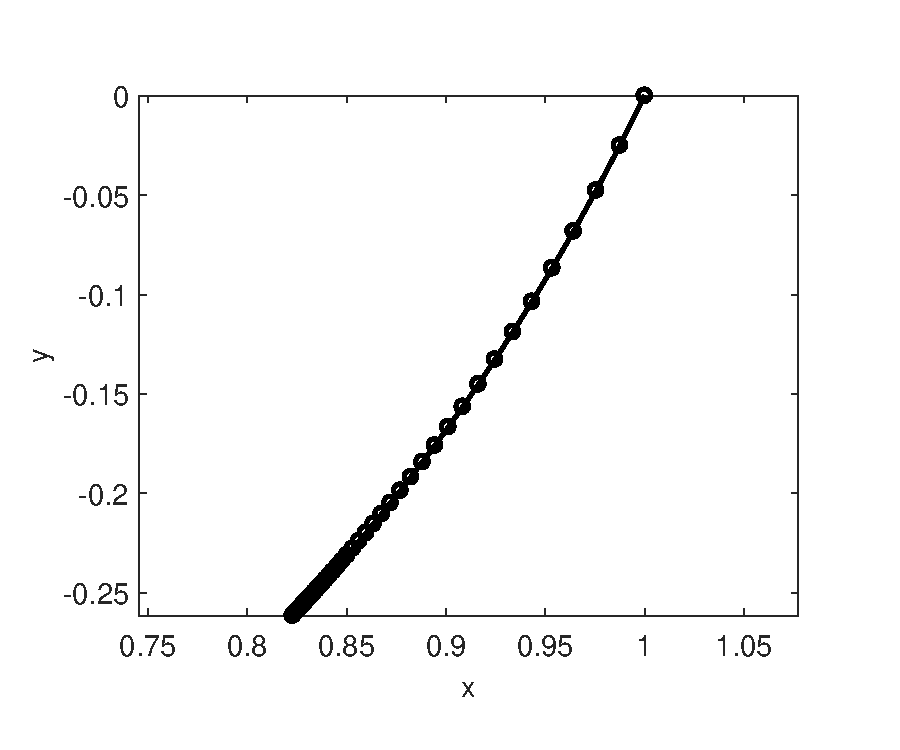
\includegraphics[width=3in]{09.matrix2/newton_raphson_2d.pdf}
\caption{Convergence of Example \ref{ex:newton_raphson_2d}. Starting at $x=1$ and $y=0$, the Newton-Raphson procedure gradually improves the output toward the root of nonlinear equation (\ref{eq:nonlinear_2d}).  The step factor $\alpha=0.1$ is used in this case.}
\label{fig:newton_raphson_2d}
\end{figure}

\end{example}

\noindent
\subsection{Broyden method: (Multidimentional Secant Method)}

In the Newton-Raphson methods, the Jacobian matrix is absolutely necessary.  However, the Jacobian matrix is not always available.  For a single variable case (See Section 3.2.3), the secant method estimates the gradient numerically.  We want to do the same here, that is to estimate the Jacobian matrix numerically.

To be written.

\section{Minimization of Mutivariable Non-Linear Functions}

We want to minimize a nonlinear function $d(\vb{x})$ with respect to $\vb{x}$.  When the gradient of $f(x)$ is known, the steepest descent or conjugate gradient method. If the gradient is not available XXXX should be used.

To be written.

\section{Applications in Physics}

\subsection{Steady states in Laser Dynamics}

In Section 4.3.2, we investigate the laser dynamics modeled by the Maxwell-Bloch equation.  Type A and B lasers reach a steady state where all variables are constant after some time. Then, the time derivatives in the Maxwell-Bloch equations vanishes, and hence
\begin{subequations}
\begin{eqnarray}
f_1 &\equiv& -\gamma_1 E + \kappa_1 P = 0 \\
f_2 &\equiv& -\gamma_2 P + \kappa_2 E D = 0 \\
f_3 &\equiv& -\gamma_3 (D-\lambda) -\kappa_3 E P = 0
\end{eqnarray}
\end{subequations}
which is a multidimensional nonlinear system.  The system has one trivial solution $E=P=0$, and $D=\lambda$.  However, when a suitable amount of energy is injected, there is another solution. (We confirmed that in Section 4.3.2.)
For type A laser with $\lambda=5$, find the nontrivial steady state values of $E$, $P$ and $D$.  In terms of mathematical terminology, this is a stable fixed point of the nonlinear dynamical system.

Let $x_1=E$, $x_2=P$, and $x_3=D$. The analytic expression of the Jacobian matrix  is given by
\begin{equation}
J = 
\begin{bmatrix}
-\gamma_1 & \kappa_1 & 0 \\ \kappa_2 D & -\gamma_2 & \kappa_2 E \\ -\kappa_3 P & -\kappa_3 E & -\gamma_3 \end{bmatrix}
\end{equation}
In Program \ref{prog:fixed_point_maxwell}, we use the multidimensional Newton-Raphson method and the Gaussian elimination with partial pivoting.
Starting with initial guess $E=2$,$P=2$, and $D=5$, the original Newton-Raphson ($\alpha=1$) experiences instability and even after a thousand iterations, the system variables are wildly changing.   When $\alpha=0.5$ is used, only several iterations (See Fig. \ref{fig:fixed_points_maxwell}.) are necessary to reach the solution which is in good agreement with the result obtained in Section 4.3.2.

\begin{figure}
\centering
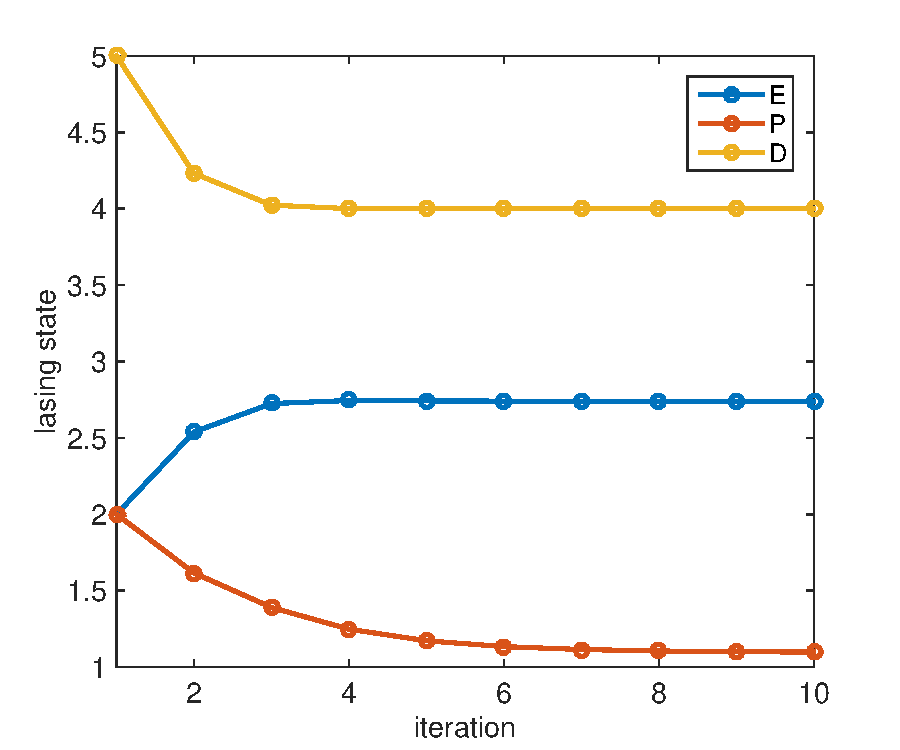
\includegraphics[width=3in]{09.matrix2/fixed_points_maxwell.pdf}
\caption{Fixed points of the Maxwell-Bloch equations for typa A laser. (See Section 4.3.2 for parameter values.)  After several iteration, the Newton-Raphson method converges to the solution.}\label{fig:fixed_points_maxwell}
\end{figure}

\newpage

\noindent
\section*{MATLAB Source Codes}
\addcontentsline{toc}{section}{\protect\numberline{}MATLAB Source Codes}

\bigskip
\noindent
\program
\label{prog:newton_raphson_2d}
\footnotesize
\begin{verbatim}
%**************************************************************************
%*     Example  9.1                                                       *
%*     filename: ch09pr01.m                                               *
%*     program listing number: 9.1                                        *
%*                                                                        *
%*     This program solves a two-dimensional non-linear equation          *
%*     by newton-raphson method.                                          *
%*                                                                        *
%*     Programed by Ryoichi Kawai for Computational Physics Course.       *
%*     Last modification:  02/04/2015.                                    *
%**************************************************************************
clear all;

% set a tolerance
tol = 1.0e-8;

% step factor (between 0 and 1)
a = 0.1;

%define functions
f1 = @(x,y) 2*x + 3*x*y - 1;
f2 = @(x,y) x*y + 3*y + 1;

%define Jacobian
J11 = @(x,y) 2+3*y;
J12 = @(x,y) 3*x;
J21 = @(x,y) y;
J22 = @(x,y) x+3;

% iniital guess
x(1) = 1;
y(1) = 0;

b(1)=-f1(x(1),y(1));
b(2)=-f2(x(1),y(1));
err=sqrt(b(1)*b(1)+b(2)*b(2));
if err < tol
    not_found = false;
else
    not_found = true;
end
n=1;

while not_found
    % Construct linear equation
    A(1,1)=J11(x(n),y(n));
    A(1,2)=J12(x(n),y(n));
    A(2,1)=J21(x(n),y(n));
    A(2,2)=J22(x(n),y(1));
    % solve the linear equation
    z=A\b;
    x(n+1)=x(n)+a*z(1);
    y(n+1)=y(n)+a*z(2);
    
    % check error
    b(1)=-f1(x(n+1),y(n+1));
    b(2)=-f2(x(n+1),y(n+1));
    err=sqrt(b(1)*b(1)+b(2)*b(2));
    fprintf('err= %f\n',err)
    if err < tol
       not_found = false;
    else
       n=n+1;
    end
end

p=plot(x,y);
set(p,'linewidth',2,'color','black')
axis equal
xlabel(texlabel('x'),'fontsize',14)
ylabel(texlabel('y'),'fontsize',14)

xa = (-1+sqrt(7))/2;
ya = (-5+sqrt(7))/9;
fprintf('Iternations = %d\n',n)
fprintf('Solution= %d, %d\n',x(n),y(n))
fprintf('   Exact= %d, %d\n',xa,ya)
\end{verbatim}
\normalsize

\ruleend
\bigskip
\noindent
\program
\label{prog:fixed_point_maxwell}
\footnotesize
\begin{verbatim}
%**************************************************************************
%*     Section  9.3.1                                                     *
%*     filename: ch09pr02.m                                               *
%*     program listing number: 9.3-1                                      *
%*                                                                        *
%*     This program finds a fixed point of Maxwell-Bloch equation         *
%*     by newton-raphson method and Gaussian elimination.                 *
%*                                                                        *
%*     Use function gauss.m                                               *
%*                                                                        *
%*     Programed by Ryoichi Kawai for Computational Physics Course.       *
%*     Last modification:  02/04/2015.                                    *
%**************************************************************************
clear all;

% system parameters
g1=0.1; g2=2; g3=3;
k1=0.25; k2=0.2; k3=1;
lambda=5;

% control parameters
alpha = 0.5;
tol = 1e-4;
N=3;

%iniital guess
y(1,1:3)=[2;2;5];
i=1;
err = 1;

x(1:3)=y(i,:);
J=[[-g1,k1,0];[k2*x(3),-g2,k2*x(2)];[-k3*x(2),-k3*x(1),-g3]];
f=[-g1*x(1)+k1*x(2);-g2*x(2)+k2*x(1)*x(3);-g3*(x(3)-lambda)-k3*x(1)*x(2)];
while err > tol
    i=i+1;
    B=gauss(J,f);
    y(i,:)=y(i-1,:) - alpha*B;
    x=y(i,:);
    J=[[-g1,k1,0];[k2*x(3),-g2,k2*x(2)];[-k3*x(2),-k3*x(1),-g3]];
    f=[-g1*x(1)+k1*x(2);-g2*x(2)+k2*x(1)*x(3);-g3*(x(3)-lambda)-k3*x(1)*x(2)];
    err = f'*f;
end

fprintf('E=%.6f,  P=%.6f,  D=%.6f\n',x)

p=plot([1:i],y(:,1),'o-',[1:i],y(:,2),'o-',[1:i],y(:,3),'o-');
set(p,'linewidth',2)
xlabel('iteration','fontsize',14)
ylabel('lasing state','fontsize',14)
legend('E','P','D')
legend('location','northeast')
\end{verbatim}
\normalsize

\ruleend
\bigskip

\footnotesize
\begin{verbatim}

%**************************************************************************
%*     Section  9.3.1                                                     *
%*     filename: gauss.m                                                  *
%*     program listing number: 9.2-2                                      *
%*                                                                        *
%*     This program solves a linear equaion Ax=b using Gaussian           *
%*     elimination and partial pivoting.                                  *
%*                                                                        *
%*     Input:  A (N x N matrix)                                           *
%*             b (N-dimensional vector)                                   *
%*                                                                        *
%*     Output: x (N-dimensional vector)                                   *
%*                                                                        *
%*     Programed by Ryoichi Kawai for Computational Physics Course.       *
%*     Last modification:  02/04/2015.                                    *
%**************************************************************************
function [x]=gauss(A,b)

% Set a linear equation
N=size(A,1);

% scale factors
for i=1:N
    S(i)=max(A(i,:));
end

for n=1:N-1
    % Look for the pivot row
    j=n;
    Amax=abs(A(n,n)/S(n));
    for i=n:N
        AS=abs(A(i,n)/S(i));
        if AS > Amax
            j=i;
            Amax = AS;
        end
    end
    % Carry out pivoting
    if j ~= n
        for i=n:N
            TMP=A(n,i);
            A(n,i)=A(j,i);
            A(j,i)=TMP;
        end
        TMP=b(n);
        b(n)=b(j);
        b(j)=TMP;
        % Record the permutation
        P(n,n)=0; P(j,j)=0;
        P(n,j)=1; P(j,n)=1;
    end
    % Gaussian elimination
    for i=n+1:N
        M=-A(i,n)/A(n,n);
        A(i,n+1:N)=M*A(n,n+1:N)+A(i,n+1:N);
        b(i)=M*b(n)+b(i);
    end
    A(n+1,n)=0;  
end

% backsubstitution
for i=3:-1:1
    Ax=0;
    for j=i+1:3
        Ax = Ax+A(i,j)*x(j);
    end
    x(i) = (b(i)-Ax)/A(i,i);
end
\end{verbatim}
\normalsize

\ruleend

\bigskip
\noindent
\section*{Python Source Codes}
\addcontentsline{toc}{section}{\protect\numberline{}Python Source Codes}
\setcounter{program}{0}

\bigskip
\noindent
\program
\footnotesize
\begin{verbatim}
# -*- coding: utf-8 -*-
"""
%**************************************************************************
%*     Example  9.1                                                       *
%*     filename: ch09pr01.py                                              *
%*     program listing number: 9.1                                        *
%*                                                                        *
%*     This program solves a two-dimensional non-linear equation          *
%*     by newton-raphson method.                                          *
%*                                                                        *
%*     Programed by Ryoichi Kawai for Computational Physics Course.       *
%*     Last modification:  02/10/2017.                                    *
%**************************************************************************
"""
import numpy as np
import matplotlib.pyplot as plt

# set a tolerance
tol = 1.0e-8

# step factor (between 0 and 1)
a = 0.1

#define functions
def f(x,y):
    return [2.0*x + 3.0*x*y - 1.0, x*y + 3.0*y + 1.0]

#define Jacobian
def J(x,y):
    return [[2.0+3.0*y,3.0*x],[y,x+3.0]]

nmax=1000
x=np.zeros(nmax+1)
y=np.zeros(nmax+1)
b=np.zeros(2)
A=np.zeros((2,2))

# iniital guess
x[0] = 1.0
y[0] = 0.0

b=-np.array(f(x[0],y[0]))

err=np.sqrt(b[0]*b[0]+b[1]*b[1])
if err < tol:
    found = True
else:
    found = False

n=0
while not(found) and n<nmax:
    
    # Construct linear equation
    A = np.array(J(x[n],y[n]))

    # solve the linear equation
    z=np.linalg.solve(A,b)
    x[n+1]=x[n]+a*z[0]
    y[n+1]=y[n]+a*z[1]
    
    # check error
    b=-np.array(f(x[n+1],y[n+1]))
    err=np.dot(b,b)
    print('err=',err)
    if err < tol:
       found = True
    else:
       n+=1


plt.figure(figsize=(6,5))     
plt.plot(x[0:n],y[0:n],'ok',linewidth=2)
plt.axes().set_aspect('equal', 'datalim')
plt.text(x[0]+0.01,y[0],'Start Here')
plt.text(x[n]+0.01,y[n]-0.01,'Converged',color='r')
plt.xlabel('x',fontsize=14)
plt.ylabel('y',fontsize=14)
plt.show()

xa = (-1.0+np.sqrt(7.0))/2.0
ya = (-5.0+np.sqrt(7.0))/9.0
print('Iternations = {0:d}'.format(n))
print('Solution= {0:f}, {1:f}'.format(x[n],y[n]))
print('   Exact= {0:f}, {1:f}'.format(xa,ya))
\end{verbatim}
\normalsize

\ruleend

\bigskip
\noindent
\program
\footnotesize
\begin{verbatim}
# -*- coding: utf-8 -*-
"""
%**************************************************************************
%*     Section  9.3.1                                                     *
%*     filename: ch09pr02.py                                              *
%*     program listing number: 9.2-1                                      *
%*                                                                        *
%*     This program finds a fixed point of Maxwell-Bloch equation         *
%*     by newton-raphson method and Gaussian elimination.                 *
%*                                                                        *
%*     Use function gauss.m                                               *
%*                                                                        *
%*     Programed by Ryoichi Kawai for Computational Physics Course.       *
%*     Last modification:  02/15/2017.                                    *
%**************************************************************************
"""
import numpy as np
import matplotlib.pyplot as plt


# system parameters
g1=0.1; g2=2.0; g3=3.0
k1=0.25; k2=0.2; k3=1.0
lam=5.0

def Jacob(x):
    J = [[-g1,k1,0.0],[k2*x[2],-g2,k2*x[1]],[-k3*x[1],-k3*x[0],-g3]]
    return J
    
def Func(x):
    f= [-g1*x[0]+k1*x[1],-g2*x[1]+k2*x[0]*x[2],-g3*(x[2]-lam)-k3*x[0]*x[1]]
    return f
            
# control parameters
alpha = 0.5
tol = 1e-4

nmax=1000
y=np.zeros((3,nmax+1))
J=np.zeros((3,3))
f=np.zeros(3)
B=np.zeros(3)

#initial guess
x=np.array([2.0,2.0,5.0])
y[:,0]=x
#y[:,0]=[x.item(0),x.item(1),x.item(2)]

n=0
err=tol+1.0
J=np.array(Jacob(x))
f=np.array(Func(x))

while err > tol and n<nmax:
    B=np.linalg.solve(J,f)
    x=y[:,n] - alpha*B
    y[:,n+1]=[x.item(0),x.item(1),x.item(2)]
    J=np.array(Jacob(x))
    f=np.array(Func(x))
    err = np.dot(f,f)
    n+=1

print('E={0:f},  P={1:f},  D={2:f}'.format(x.item(0),x.item(1),x.item(2)))
print('err=',err)

t=np.linspace(0,n,n+1)
plt.figure()
plt.plot(t,y[0,0:n+1],'-ok',label='E')
plt.plot(t,y[1,0:n+1],'-ob',label='P')
plt.plot(t,y[2,0:n+1],'-or',label='D')
plt.xlabel('iteration')
plt.ylabel('lasing state')
plt.xlim(0.,9.)
plt.ylim(0.,6.)
plt.legend(loc=1)
plt.show()
\end{verbatim}

\normalsize

\ruleend

\newpage
%\chapbibliography
\bibliographystyle{unsrt}
\bibliography{compphys}